\documentclass[
  a4paper,            % DIN A4
  DIV=10,             % Schriftgröße und Satzspiegel
  oneside,            % einseitiger Druck
  BCOR=5mm,           % Bindungskorrektur
  parskip=half,       % Halber Abstand zwischen Absätzen
  numbers=noenddot    % Kein Punkt hinter Kapitelnummern
]{scrreprt}
\usepackage{../style/thesisstyle}

%---------------------------------------
\usepackage{url}
\usepackage{subcaption,graphicx}
\usepackage{interval}

\usepackage{siunitx}
\sisetup{quotient-mode=fraction}

\newcommand\note[1]{\textcolor{red}{#1}} % text within the \note command will be red (implicating a TODO)

\usepackage[labeled]{multibib}             %% ermöglicht mehrere Literaturverzeichnisse (inkl. unterschiedl. Zitatkennzeichnung)
\newcites{I}{Internetquellen}    %% Umbenennen der zusätzlichen Verzeichnisse
%---------------------------------------
\makeglossaries           % create all glossary entries (remember: run makeglossaries manually)
\loadglsentries{thesisglossaries.tex}  % load acronym, symbol and glossarie entries

\begin{document}
% !TEX root = ../thesis.tex
%
% configurations
%

% text field
%-> replace supervisor names with correct ones
\firstSupervisor{Prof. Dr.-Ing. Andreas Meisel}
\secondSupervisor{Prof. Dr. rer.nat. Stephan Pareigis}

% text field
%-> replace title with your thesis title
\thesisTitle{Bildbasierte Navigation mit Neuronalen Netzen}
\thesisTitleEN{Image based navigation with Neural Networks}

% text field
%-> replace the key words with your own key words
\keywordsDE{Leben, Universum, Alles}
\keywordsEN{Life, Universe, Everything}

% text field
%-> replace the text with a description of the thesis
\abstractDE{In dieser Bachelorarbeit soll untersucht werden, wie Navigation auf reinen Bildaten funktionieren kann. Konkret geht es um das Erkennen einer Fahrbahn mit einem Neuronalen Netz, bzw. um das Erzeugen von Lenkwinkeldaten auf Basis eines Bildes einer Fahrbahn. Hierzu wird ein trainiertes Neuronales Netz mittels Fine Tuning abgestimmt.  Das wid direkt zur Anwendung gebracht auf einem RC Fahrzeug aus dem "Carolo-Cup", inklusive Fahrten auf einer Teststrecke. }
\abstractEN{Arthur Dents travel to a new future \dots}

% text field
%-> replace jon with your name
\thesisAuthor{Jan Robert Rösler}

% text field
%-> enter the submission date
\submissionDate{07. Juni 1954}

% switch - uncomment only one
%-> uncomment NDA or public
%\NDA{yes}
\NDA{no}

% switch - uncomment only one
%-> uncomment to show list of figures or not 
\ListOfFigures{yes}
%\ListOfFigures{no}

% switch - uncomment only one
%-> uncomment to show list of tables or not 
\ListOfTables{yes}
%\ListOfTables{no}

% switch - uncomment only one
%-> uncomment to show list of accronyms or not 
\ListOfAccronyms{yes}
%\ListOfAccronyms{no}

% switch - uncomment only one
%-> uncomment to show list of symbols or not 
\ListOfSymbols{yes}
%\ListOfSymbols{no}

% switch - uncomment only one
%-> uncomment to show list of glossary entries or not 
\Glossary{yes}
%\Glossary{no}

% switch - uncomment only one
%-> uncomment the study course you are in
%\studycourse{ITS}
\studycourse{TI}
%\studycourse{AI}
%\studycourse{WI}
%\studycourse{EI}
%\studycourse{BMT}
%\studycourse{MAI}
%\studycourse{MIK}
%\studycourse{MA}
    % load all settings

\hyphenation{Ba-che-lor-the-sis Mas-ter-the-sis}

% Cover page here, no page number
% !TEX root = ../thesis.tex
%
% cover page
% @author Thomas Lehmann
%

\thispagestyle{empty}
\begin{titlepage}
{\fontfamily{phv}\selectfont

% NDA, if needed
  \hfuzz=20pt
\begin{textblock*}{\textwidth}(75mm,9mm)
  \begin{minipage}[b][0cm][b]{\textwidth}
  \hfuzz=20pt
  \fontsize{16pt}{16pt}
  \selectfont
    \begin{flushleft}
    	  \IthesisNDAFull
    \end{flushleft}
  \end{minipage}
\end{textblock*}

% black-white logo
\begin{textblock*}{\textwidth}(134mm,40mm)
  \begin{minipage}[b][0cm][b]{\textwidth}
    
\includegraphics[scale=0.5]{../style/HAW_Marke_schwarz}
  \end{minipage}
\end{textblock*}

% kind of thesis
\begin{textblock*}{\textwidth}(30mm,115mm)
  \begin{minipage}[b][0cm][b]{\textwidth}
    \fontsize{22pt}{20pt}
    \selectfont
  	\begin{flushright}
      \IthesisKind
  	\end{flushright}
  \end{minipage}
\end{textblock*}

% author of thesis
\begin{textblock*}{\textwidth}(30mm,140mm)
  \begin{minipage}[b][0cm][b]{\textwidth}
  \fontsize{14pt}{20pt}
  \selectfont
    \begin{flushright}
      \IthesisAuthor
  	\end{flushright}
  \end{minipage}
\end{textblock*}

% Title of thesis
\begin{textblock*}{\textwidth}(30mm,155mm)
  \begin{minipage}[b][0cm][t]{\textwidth}
  %\fontsize{18pt}{20pt}
  \ITitleFontSize
  \selectfont
  	\begin{flushright}
       \IthesisTitle
  	\end{flushright}
  \end{minipage}
\end{textblock*}

\ITextBlockSupervisionOnCover

% german version of faculty and department
\begin{textblock*}{\textwidth}(20mm,256mm)
  \begin{minipage}[b][0cm][t]{\textwidth}
  \fontsize{11pt}{10pt}
  \selectfont
    \begin{flushleft}
      \textit{\IthesisFacultyFull} \\
      \textit{\IthesisDepartmentFull}
    \end{flushleft}
  \end{minipage}
\end{textblock*}

% english version of faculty and department
\begin{textblock*}{\textwidth}(52mm,256mm)
  \begin{minipage}[b][0cm][t]{\textwidth}
  \fontsize{11pt}{10pt}
  \selectfont
    \begin{flushright}
      \textit{\IthesisFacultyFullEN} \\
      \textit{\IthesisDepartmentFullEN}
    \end{flushright}
  \end{minipage}
\end{textblock*}
}
\end{titlepage}
\                % this backslash is needed, otherwise LaTeX does wired things ....


% Titlepage is page one even if the number is not shown.
\pagenumbering{roman}
% Title page here
% !TEX root = ../thesis.tex
%
% title page
% @author Thomas Lehmann
% Hints for titel page and page numbering: https://en.wikipedia.org/wiki/Title_page
%
\newpage
\thispagestyle{empty}
{\fontfamily{phv}\selectfont
  \hfuzz=20pt       % suppress warnings due to extenstion onto page margins

  % Author of thesis
  \vspace*{1cm}
  \begin{minipage}[b]{\textwidth}
    \fontsize{14pt}{20pt}
    \selectfont
    \begin{center}
      \IthesisAuthor
    \end{center}
  \end{minipage}

  % Title of thesis
  \vspace{1.5cm}
  \begin{minipage}[b][0cm][t]{\textwidth}
    \fontsize{18pt}{20pt}
    \selectfont
    \begin{center}
      \IthesisTitle
    \end{center}
  \end{minipage}

  % Important information
  \begin{textblock*}{\textwidth}(40mm,210mm)
    \begin{minipage}[b]{\textwidth}
      \hbadness=10001    % suppress underfull warning due to short text
      \fontfamily{cmr}\selectfont
      \fontsize{12pt}{14pt}
      \selectfont
      \IthesisKindDE ~eingereicht im Rahmen der \IthesisExaminationDE \\
      im Studiengang \IstudyCourseName \\
      am \IthesisDepartmentFull \\
      der Fakultät Technik und Informatik\\
      der Hochschule für Angewandte Wissenschaften Hamburg\\

      Betreuender Prüfer: \IfirstSv \\
      Zweitgutachter: \IsecondSv \\

      Eingereicht am: \ISubDate \\
    \end{minipage}
  \end{textblock*}
}


% Abstract page here
% !TEX root = ../thesis.tex
%
% abstract page
% @author Thomas Lehmann
%
\newpage
\thispagestyle{plain}
\clearpage
\hfuzz=12pt       % suppress warnings due to extenstion onto page margins

\textbf{\IthesisAuthor}

\vspace{0.5cm}
\textbf{Thema der Arbeit}

\IthesisTitle

\vspace{0.3cm}
\textbf{Stichworte}

\IkeyWordsDE

\vspace{0.3cm}
\textbf{Kurzzusammenfassung}

\begin{minipage}{\textwidth}
\IabstractDE
\end{minipage}

\vspace{1.0cm}
\textbf{\IthesisAuthor}

\vspace{0.3cm}
\textbf{Title of Thesis}

\IthesisTitleEN

\vspace{0.3cm}
\textbf{Keywords}

\begin{minipage}{\textwidth}
\IkeyWordsEN
\end{minipage}

\vspace{0.3cm}
\textbf{Abstract}

\IabstractEN


% Table of contents here
\tableofcontents

% List of figures here
\IListOfFigures

% List of tables here
\IListOfTables

% List of accronyms here
\IListOfAccronyms

% List of symbols here
\IListOfSymbols

% Uncomment if list of source code is needed (rarely).
%\lstlistoflistings  % requires package listings, needs to uncommenting of usepackage

% path to the chapters folder is set to find the images used there
\graphicspath{ {./chapters/} }

% Chapters
\clearpage
\pagenumbering{arabic}
% first example chapter
% @author Jan Robert Rösler 
%


\chapter{Einleitung}


Sobald ein System, welcher Art sei offen, mobil wird, also läuft, rollt, gleitet, schwebt oder schwimmt, steht es vor der Aufgabe der Navigation. Das kann zunächst bedeuten, zu Wissen, wo es sich befindet. Auf einer Karte oder auch relativ zu anderen "Dingen"  in der Umgebung. Weiter können sich dann Fragen der Pfadplanung stellen, je nach Ziel oder Aufgabe des mobilen Systems. Ebenfalls könnte es dann von Interesse zu sein, eine eigene Repräsentation (oder Interpretation) der Umgebung aufzubauen und zu speichern, um Lokalisation und Pfadplanung kontinuierlich zu betreiben. Je nach Art und Aufgabe des Systems sind konkrete Probleme in der Navigation und ihre Lösungen zum Beispiel \note{(NAVIGATIONSPRBLEME UND LOESUNG KLASSISCH)} //


\section{Autome Navigation}





% @author Jan Robert Rösler 
%
\chapter{Neuronale Navigation mit Bilddaten}

\section{Relevante Technik/Hintergrund}
Hier erfolgt zunächst eine kurze Beschreibung der für Neuronale Navigation auf Bilddaten relevanten Technik. Grundlegendes wird nur der Vollständigkeit halber erwähnt, speziellere Aspekte kurz vorgestellt. 

\subsection{Deep Learning}

\subsection{CNN}
\textit{Convolutional Neural Networks}, oder kurz CNN, haben sich gerade im Bereich der Bildverarbeitung als überlegen bewiesen. Aus der Biologie inspiriert, findet hier besonders das Prinzip des rezeptiven Feldes Anwendung. Die Aktivität jedes Neurons wird mithilfe einer Faltung berechnet, räumliche Informationen und Zusammenhänge werden so besser erhalten. 2012 konnte ein CNN, AlexNet \cite{krizhevsky2012imagenet}, beim ImageNet-Wettbewerb den Benchmark-Rekord von 25,8 \% auf 16,4 \% drücken, seitdem sind alle gut platzierten Modelle CNNs.
CNNs sollen hier nicht detailliert erklärt werden, das Verständnis wird als Grundlage vorausgesetzt.

\subsection{ResNet}
\textit{Residual Neural Networks}, oder kurz ResNet, ist eine weitere Technik, die ihren Urprung in der Biologie hat. Verhalten so genannter Pyramidenzellen, Nervenzellen im menschlichen Gehirn, wird nachgebildet, indem Abkürzungen zwischen Layer eingebaut werden. Residual Netze wurden 2015 entwickelt, insbesondere ließ sich mit diesem Ansatz das trainieren tiefer Netze verbessern \cite{DBLP:journals/corr/HeZRS15}. \ref{img:ResBlock} zeigt den schematischen Aufbau eines so genannten Residual Blocks. 


\begin{figure}
	\centering
	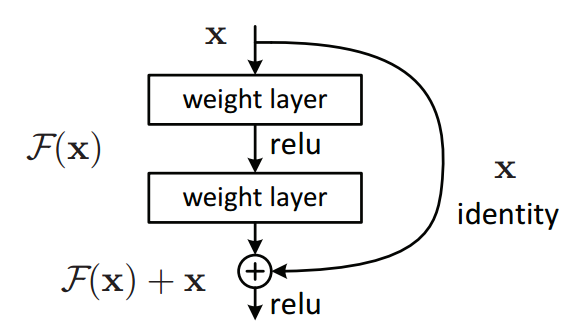
\includegraphics[scale=0.5]{figures/ResidualBlock.png}
	\caption{Residual Block}
	Quelle: \citeI{ResBlock}
	\label{img:ResBlock}
\end{figure}


DBLP:journals/corr/HeZRS15

\subsection{Fine tuning}
LAYER FREEZING 
Fine Tuning 









\section{Ansätze}
Im folgenden wird auf zwei Ansätze der Navigation mit Neuronalen Netzen eingegangen, durch Gegenüberstellung erster Versuche mit einem modernen Ansatz soll folgenden Ausarbeitungen ein Rahmen gegeben werden.

\subsection{ALVINN}

Versuche durch neuronale Verarbeitung von reinen Bilddaten in einem Szenario zu navigieren, gab es bereits 1989 in Pomerleau's Arbeit, die man auf diesem Gebiet als Pionierarbeit verstehen kann.\cite{pomerleau1989alvinn}.
Das Netzwerk ALVINN (Autonomous Land Vehicle In a Neural Network) sollte das NAVLAB steuern, ein Testfahrzeug für Autonome Navigation der Carnegie Mellon University.
In \ref{img:ALVINNa} lässt sich die Architektur nachvollziehen. 
Der rein visuelle Input (die Blautstufenintensität eines Pixels bestimmt das Aktivierungslevel des Inputneurons) wird untersützt durch eine laserbasierte Abstandsmessung und ein Inputneuron für die Kodierung der \glqq Straßenintensität\grqq{}, also ob die Straße heller oder dunkler wird.
Aus heutiger Sicht ist das Netz mit nur einer hidden Layer mit 29 Neronen sehr klein, die im weiteren angesprochenen Architekturen haben deutlich mehr Layer und mehrere Hunderttausend Parameter. 
Zudem interpretiert ALVINN die Aufgabe des Spurfolgens nicht als Regressionsproblem, sondern als Klassifikation. Die Ausgangsneuronen sind eine lineare Repräsentation der Lenkrichtung, die das Fahrzeug in Richtung Fahrbahnmitte steuert. Neuronen in der Mitte stehen für eine Fahrt geradeaus, Neuronen links und rechts für die jeweilige Fahrtrichtung.
Grob gesagt gibt das Neuron mit dem höchsten Aktivierungslevel die Fahrtrichtung (den einzuschlagenden Lenkwinkel) an.
Im Ergebnis konnte das Netz nach 40 Epochen Training auf simulierten Fahrbahnbildern, zu sehen in \ref{img:ALVINNb}, einen 400 Meter Weg durch einen Wald mit \SI{1/2}{\meter/\second} sicher abfahren.//

\begin{figure}
	\centering
	\begin{subfigure}{.5\textwidth}
	\centering
		  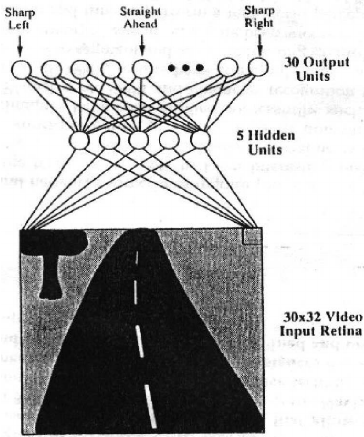
\includegraphics[width=.85\linewidth]{figures/Architecture-ALVINN.png}
		  \caption{}
		  \label{img:ALVINNa}
	\end{subfigure}%
	\begin{subfigure}{.5\textwidth}
	\centering
		  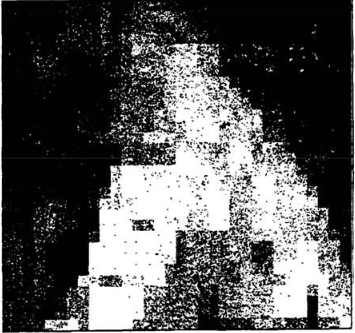
\includegraphics[width=.85\linewidth]{figures/Strasse-ALVINN.png}
	 	  \caption{}
		  \label{img:ALVINNb}
	\end{subfigure}%
	\caption{ALVINN Architektur (a) und simulierte Fahrbahn (b)}
	%Quelle: \protect\citeI{Architecture-ALVINN}
	\label{img:ALVINN}
\end{figure}

\subsection{NVIDIA DAVE-2}

Forschungserkenntnisse der folgenden Jahre trieben die Entwicklung voran und...
Im Jahr 2016 veröffentlicht das Technologieunternehmen \textsc{NVIDIA} einen eigenen Ansatz \cite{bojarski2016end}, basierend auf Versuchen mit dem \glqq DARPA Autonomous Vehicle \grqq{} (DAVE) \citeI{DarpaDave} wird dieser \glqq Dave-2 \grqq{} genannt.//
Daten werden hier durch Fahrten auf echten Straßen gesammelt, wofür drei Kameras in der Windschutzscheibe eines Autos angebracht und Steuerungsdaten über den CAN-Bus des Fahrzeuges ausgelesen werden. Mit diesen Daten wird ein CNN trainiert \ref{img:NVIDIA}, was dann an einer Straßen-Simulation getestet wird. Hervorzuheben ist hier besonders die Verwendung von Convolutional Neural Networks (CNN) und die, im Gegensatz zum bereits erwähnten Ansatz 27 Jahre zuvor, stark gesteigerte Rechenleistung. Folglich können nicht nur Bilder besserer Qualität verarbeitet werden, die Netzarchitektur mit 9 Layern und 250.00 Parametern wäre 1989 nicht in annehmbarer Zeit trainierbar gewesen. Außerdem stellt sich NVIDIA dem Anspruch, eine neuronale Steuerung für öffentliche Straßen zu entwerfen, nicht nur für ein sehr begrenztes Testszenario.



\begin{figure}
	\centering
	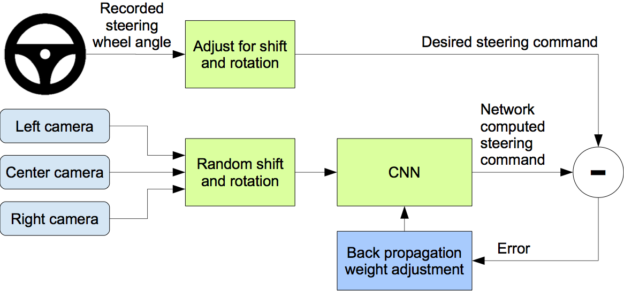
\includegraphics[scale=0.5]{figures/NVIDIA-Training.png}
	\caption{Komponenten des Trainings}
	Quelle: \citeI{NVIDIA-Components}
	\label{img:NVIDIA}
\end{figure}





 Präsentation ALVINN, dann gegenüberstellung mit modernem Netzwerk a la NVIDIA.






Kurzer Blick auf  Self driving car steering angle4 prediction und berkeley (large scale video sets) (vielleicht auchSPÄTER)




Glossar

Convolutional Neural Network CNN



% first example chapter
% @author Jan Robert Rösler 
%
\chapter{Idee}

\section{DroNet und Carolo-Cup}

Die \gls{gl:eth} entwickelte 2018 eine eigene Architektur, mit dem Ziel durch Training auf Fahrbahnbildern eine Drone zu steuern \cite{Loquercio_2018}. 
Das daraus entstandene, von Aufbau und Größe relativ einfach gehaltene Neuronale Netz, war der Anstoß für diese Arbeit. 

Das Netz, siehe Abbildung~\ref{img:DroNet}, bekommt als Input ein 200x200 Pixel großes Bild in Graustufen, der Output ist ein Lenkwinkel und zusätzlich eine Kollisionswahrscheinlichkeit.\\

\begin{figure}[h]
	\centering
	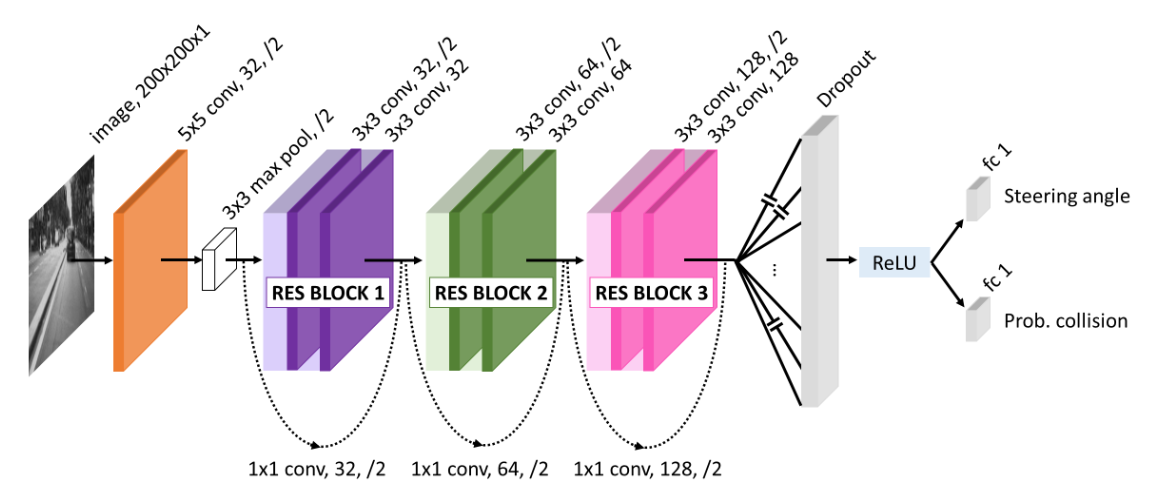
\includegraphics[scale=0.5]{figures/Architecture-DRONET.png}
	\caption{Architektur \textsc{DroNet}}
	\label{img:DroNet}
\end{figure}

Trainiert wurde das Netz auf frei verfügbaren Datensätzen der Firma \gls{gl:udacity}, bestehend aus Bildern aufgenommen mit Kameras hinter der Windschutzscheibe eines Autos bei stundenlagen Fahrten über Amerikanische Highways. Die Aufnahmen sind mit Fahrdaten verbunden, Zeitstempel, GPS-Daten, Beschleunigungswerte und Lenkwinkel wurden für jedes Bild der Aufnahmen gespeichtert. Für das Training von \textsc{\gls{gl:dronet}} werden nur die Bilder der Mittelkamera und der jeweilige Lenkwinkel genutzt.\\
Zusätzlich hat das Team der ETH Zürich eigene Aufnahmen mithilfe einer am einem Fahrrad montierten Kamera im Straßenverkehr gemacht und diese Aufnahmen manuell mit einer Kollisionswahrscheinlichkeit versehen. Wie bereits erwähnt hat das Netzwerk dementsprechend zwei verschiedene Outputs.\\
Für diese Arbeit ist aber nur der Lenkwinkel von Interesse, Kollision spielt als Szenario keine Rolle. Im Entwurf werden dementsprechend Anpassungen gemacht.

Es stellte sich heraus, dass das Modell hervorragend generalisierte und eine Drohne sicher durch ein Straßenszenario steuern konnte, wobei das Szenario sich deutlich von den gelernten Unterschied. Diese Eigenschaft von \textsc{DroNet} möchte ich mir im folgenden zu Nutze machen und auf dieser Basis ein Steuerungsmodell für ein RC-Fahrzeug entwickeln.\\

Die \gls{gl:haw} nimmt bereits seit einigen Jahren am \glqq \gls{gl:carolo} \grqq{} teil, einem Wettbewerb der Technischen Universität Braunschweig. Hier treten Teams einiger deutscher Hochschulen mit RC-Fahrzeugen (Maßstab 1:10) in verschiedenen Disziplinen des autonomen Fahrens gegeneinander an. Der Wettbewerb findet jährlich in Braunschweig auf einem vorbereiteten Kurs statt.
Eine hauptsächlich von den HAW Studenten Nils Schönherr und Gunnar Wolfram aufgebaute Plattform, zu sehen in Abbildung~\ref{img:Carolo-Fahrzeug}, dient dieser Arbeit als Testplattform.

\begin{figure}[h]
	\centering
	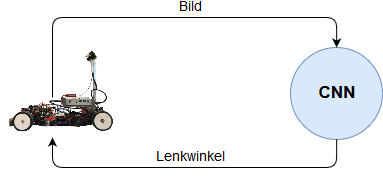
\includegraphics[scale=0.7]{figures/Aufbau.png}
	\caption{Einfacher schematischer Aufbau }
	\label{img:Aufbau}
\end{figure}


Zum entwickeln der Fahrzeuge steht an der HAW eine Teststrecke zur Verfügung, verschiedene Fahrzeugplattformen sind in der Entwicklung.\\
Das Ziel dieser Bachelorarbeit ist, an einem konkreten Anwendungsfall zu zeigen, dass ein Fahrzeug autonom einen Streckenkurs abfahren kann, indem ein neuronales Netz live Bilder der Strecke auswertet und Lenkinformationen für das Fahrzeug berechnet, schematisch dargestellt in Abbildung~(\ref{img:Aufbau}). Da aktive Teams der HAW im Carolo-Cup aktuell klassische (Bildbasierte-) Navigationsansätze verfolgen (Kapitel~\ref{sec:Autonome Navigation mit Bilddaten}), soll die Arbeit auch zeigen, wie eine nächste Generation der Fahralgorithmen für den Carolo-Cup aussehen kann.\\

Die autonome Fahrleistung auf der Teststrecke ist das Hauptaugenmerk, sie zu messen ist zu analysieren ist Bestandteil der Arbeit.




% first example chapter
% @author Jan Robert Rösler 
%
\chapter{Entwurf}


Änderungen an der Architekrtur des Netzes
Lernarchitekrur (Pipepline)
Steuerungsarchitektur
Bilder mit Steuerdaten (Verarbeitungspipelone)
Fahrzeug (Kamera, Rechner etc.)
Strecke 
Training 
Performance (Rechenzeit) bei prediction auf dem Fahrzeug
Kommunikation zwischen C und pYthon
% first example chapter
% @author Jan Robert Rösler 
%
\chapter{Auswertung und Szenarien}
In diesem Kapitel wird der Traningsprozess analysiert und kritisch Bewertet, zudem wird das entworfene neuronale Steuerungssystem einem Test unterzogen. Verschiedene Fahrszenarien werden untersucht, zum Schluss bietet eine grafische Auswertung einen Einblick in die Perspektive aus Sicht des neuronalen Netzes.

\section{Training}
Das Fine-Tuning wurde mit den im vorangegangenem Kapitel festgelegten Konfigurationen durchgeführt. In diesem Abschnitt erfolgt eine Betrachtung des erfolgten Tranings. In Abbildung:~\ref{img:loss} sind Traningsfehler und Validierungsfehler (y-Achse) über $100$ Epochen (x-Achse) dargestellt. 

\begin{figure}[h]
	\centering
	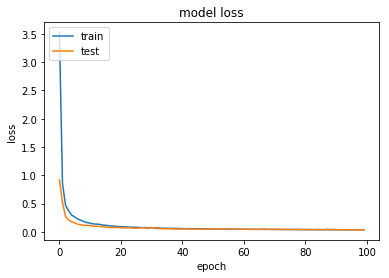
\includegraphics[scale=0.7]{figures/loss.png}
	\caption{Traningsfehler (train) und Validierungsfehler (val) über 100 Epochen}
	\label{img:loss}
\end{figure}

Festzustellen ist, dass beide Fehlerwerte sich zunächst stark fallend $0.0$ annähren und zwischen den Epochen $20-25$ und $100$ gleichbleibend $0.0$ zu sein scheinen. Aufgrund der Start-Traningsfehler von etwa $3.5$ lassen sich sehr kleine Werte nicht grafisch beurteilen. Ein direkter Blick auf die Fehlerwerte zeigt, dass beide sich im Bereich \num{10e-2} weiter $0.0$ annähern, mit dem Besten Validierungsfehler von $0.0344$ in Epoche $197$. Es besteht keine ausgeprägte Divergenz zwischen Trainings- und Validierungsfehler, das ist positiv zu beurteilen.

Bei kritischer Betrachtung muss angemerkt werden, dass die Regressionkurve, im konkreten Fall die Annäherung des Lenkwinkels, sehr rapide fällt.  Dieses kann Zeichen eines Overfittings sein. Die Bilder der Teststrecke könnten in der Menge zu homogen sein, die Teststrecke ist im Angesicht der dort aufgenommenen Bildermenge relativ kurz, viele Bilder sind ähnlich mit nur leicht unterschiedlichen Lenkwerten. Aufgrund der räumlichen Abgeschlossenheit der Teststrecke gibt es dazu wenig Varianz im Bildhintergrund, das könnte die Gleichartigkeit der Bilder verstärken.

Allerdings ist die schnelle Konvergenz nicht zwingend negativ anzumerken, das neuronale Netz war schließlich schon mit derselben Aufgabe auf einer ähnlichen Bildermenge trainiert worden. Dazu kommt, dass nur ein Teil der Layer überhaupt für das Traning, also eine Veränderung der Gewichte, freigegeben war. Im Angesicht dieser Umstände, können die Fehlerkurven in Abbildung~\ref{img:loss} auch für eine schnelle, effiziente Anpassung der Gewichte des letzten Residual-Blocks stehen.

Wie das CNN als Steuerungslogik in realen Streckenszenarien abschneidet, wird in den nächsten Abschnitten untersucht.

\section{Testfahrt}
Um die Lenkwinkelbestimmung des Netzes zu Testen, wird zunächst frei auf der Strecke gefahren. Das Fahrzeug startet auf einer Geraden und fährt den Kurs überwiegend Fehlerfrei ab. Der Onboard-Rechner (NUC) des Fahrzeugs verarbeitet die Bilder mit $20 fps$, getestet wird bis zu einer Geschwindigkeit von \SI{1.2}{\meter/\second}, ab da nimmt die Lenkfehlerhäufigkeit stark zu. Ein Lenkwinkelupdate (verarbeiteter Frame) pro gefahrene $6 cm$ ist zum sauberen Fahren die Grenze.\\
\paragraph{Autonomiemetrik}
Die Fahrleistung auf der Strecke soll gemessen werden, um Sie direkt mit anderen Algorithmen vergleichen zu können. Dazu wird eine Autonomie-Metrik bestimmt \cite{bojarski2016end}. Der Autonomiewert wird definiert als 
\begin{equation}
\label{mat:autonomie}
(1 -  \frac{\text{Anzahl Fehler}\cdot 2 s}{\text{Fahrzeit in Sekunden}})\cdot 100,
\end{equation}
wobei die Anzahl der Fehler die Summe der Situationen ist, in der das Fahrzeug die Außen- oder Mittellinie mit mehr als zwei Reifen überquert hat. Das Fahrzeug kann sich danach selbst wieder auf die Strecke bringen, oder per Hand zurückgelenkt werden. Die Zeit, die vergeht, bis das Fahrzeug wieder sauber auf die Straße zurückgekehrt ist, wird mit 2 Sekunden angenommen. Die Fahrzeit in Sekunden beschreibt die Dauer des Versuchs.

Für den Test werden zwei Runden auf der Teststrecke gefahren, einmal im Uhrzeigersinn und einmal gegen den Uhrzeigersinn, beide Runden auf der jeweils Rechten Straßenseite. Als Geschwindigkeit wird \SI{1/2}{\meter/\second} festgelegt. In jede Richtung der Strecke wird $60$ Sekunden gefahren, das entspricht je einer Runde. Die Gesamtfahrzeit für alle Tests ist damit $120$ Sekunden.

Verglichen wird das unveränderte DroNet, die abgestimmte (finegetunte) Variante (bezeichnet als BA-RR) und der Steuerungsalgorithmus (Linienerkennung), der von der diesjährigen Carolo-Cup-Projektgruppe entwickelt wurde. Die erste Runde ist mit, die zweite gegen den Uhrzeigersinn. Die Testfahrten ergaben die in Tabelle~\ref{tab:testfahrten} gesammelten Daten.



\begin{table}[h]
  \begin{center}
    \caption{Algorithmen im Vergleich}
    \label{tab:testfahrten}
    \begin{tabular}{l|c|r} % <-- Alignments: 1st column left, 2nd middle and 3rd right, with vertical lines in between
      \textbf{Algorithmus} & \textbf{Fehler Runde 1} & \textbf{Fehler Runde 2}\\
      \hline
      DroNet & 16 & 12\\
      Carolo-Projekt & 7 & 11\\
       BA-RR& 3 & 5\\
    \end{tabular}
  \end{center}
\end{table}

Der Autonomiewert wird nach der Formel berechnet und liefert die in Tabelle~\ref{tab:autonomie} vermerkten Werte. Der Autonomiewert ist eine Prozentangabe und ist auf ganze Zahlen gerundet.

\begin{table}[h]
  \begin{center}
    \caption{Vergleich der Autonomie}
    \label{tab:autonomie}
    \begin{tabular}{l|r} % <-- Alignments: 1st column left, 2nd middle and 3rd right, with vertical lines in between
      \textbf{Algorithmus} & \textbf{Autonomiewert} \\
      \hline
      DroNet & 53 \% \\
      Carolo-Projekt & 70 \%  \\
       BA-RR& 87 \% \\
    \end{tabular}
  \end{center}
\end{table}

Der ursprüngliche DroNet Algorithmus ist nur $53 \%$ der Fahrzeit autonom unterwegs, was nicht überrascht, da er in einem anderen Anwendungsszenario entstand. Der Algorithmus des aktuellen Carolo-Projektteams ist deutlich besser, hat allerdings auch viele Fahrfehler gemacht. Die in dieser Arbeit entwickelte Steuerung (BA-RR) ist $87 \%$ der Fahrzeit autonom unterwegs, hier zeigt sich die deutliche Verbesserung, die insbesondere im Gegensatz zum DroNet Algorithmus erreicht wurde. Außerdem wird deutlich, das eine Steuerung mittels statistischer Auswertung von Bilddaten (CNN) nicht nur möglich ist, sondern einer Steuerung mittels klassicher Linienerkennung sogar überlegen sein kann. 

Im Folgenden wird das Verhalten des Fahrzeugs in bestimmten Szenarien untersucht.

\section{Einzelszenarien}

\paragraph{Fahrbahn wiederfinden}
Im Hinblick auf die Eingangs angesprochene mögliche Overfitting-Problematik, wird hier eine praktische Herangehensweise an die Analyse gemacht.
Im Traningsbilderset sind keine Bilder enthalten, in denen das Fahrzeug aus einer Fehlersituation wieder auf die Straße navigiert. Genauer gesagt, in denen das Fahrzeug nicht oder nur teilweise auf der Strecke steht und den Weg in die richtige Fahrspur selbst findet. Somit konnten diese Szenarien beim Traning auch nicht \glqq auswendig \grqq{} gelernt werden. Diese Fehlersituationen werden jetzt künstlich erzeugt und das Fahrverhalten betrachtet.
Abbildung~\ref{fig:fehlerszenarien} zeigt Beispielhaft zwei solche Szenarien, einmal steht das Fahrzeug teilweise auf der Straße (\ref{fig:szena}), im anderen Beispiel steht es komplett außerhalb der Fahrbahn (\ref{fig:szenb}).


\begin{figure}[h]
	\centering
	\begin{subfigure}{.5\textwidth}
	\centering
		  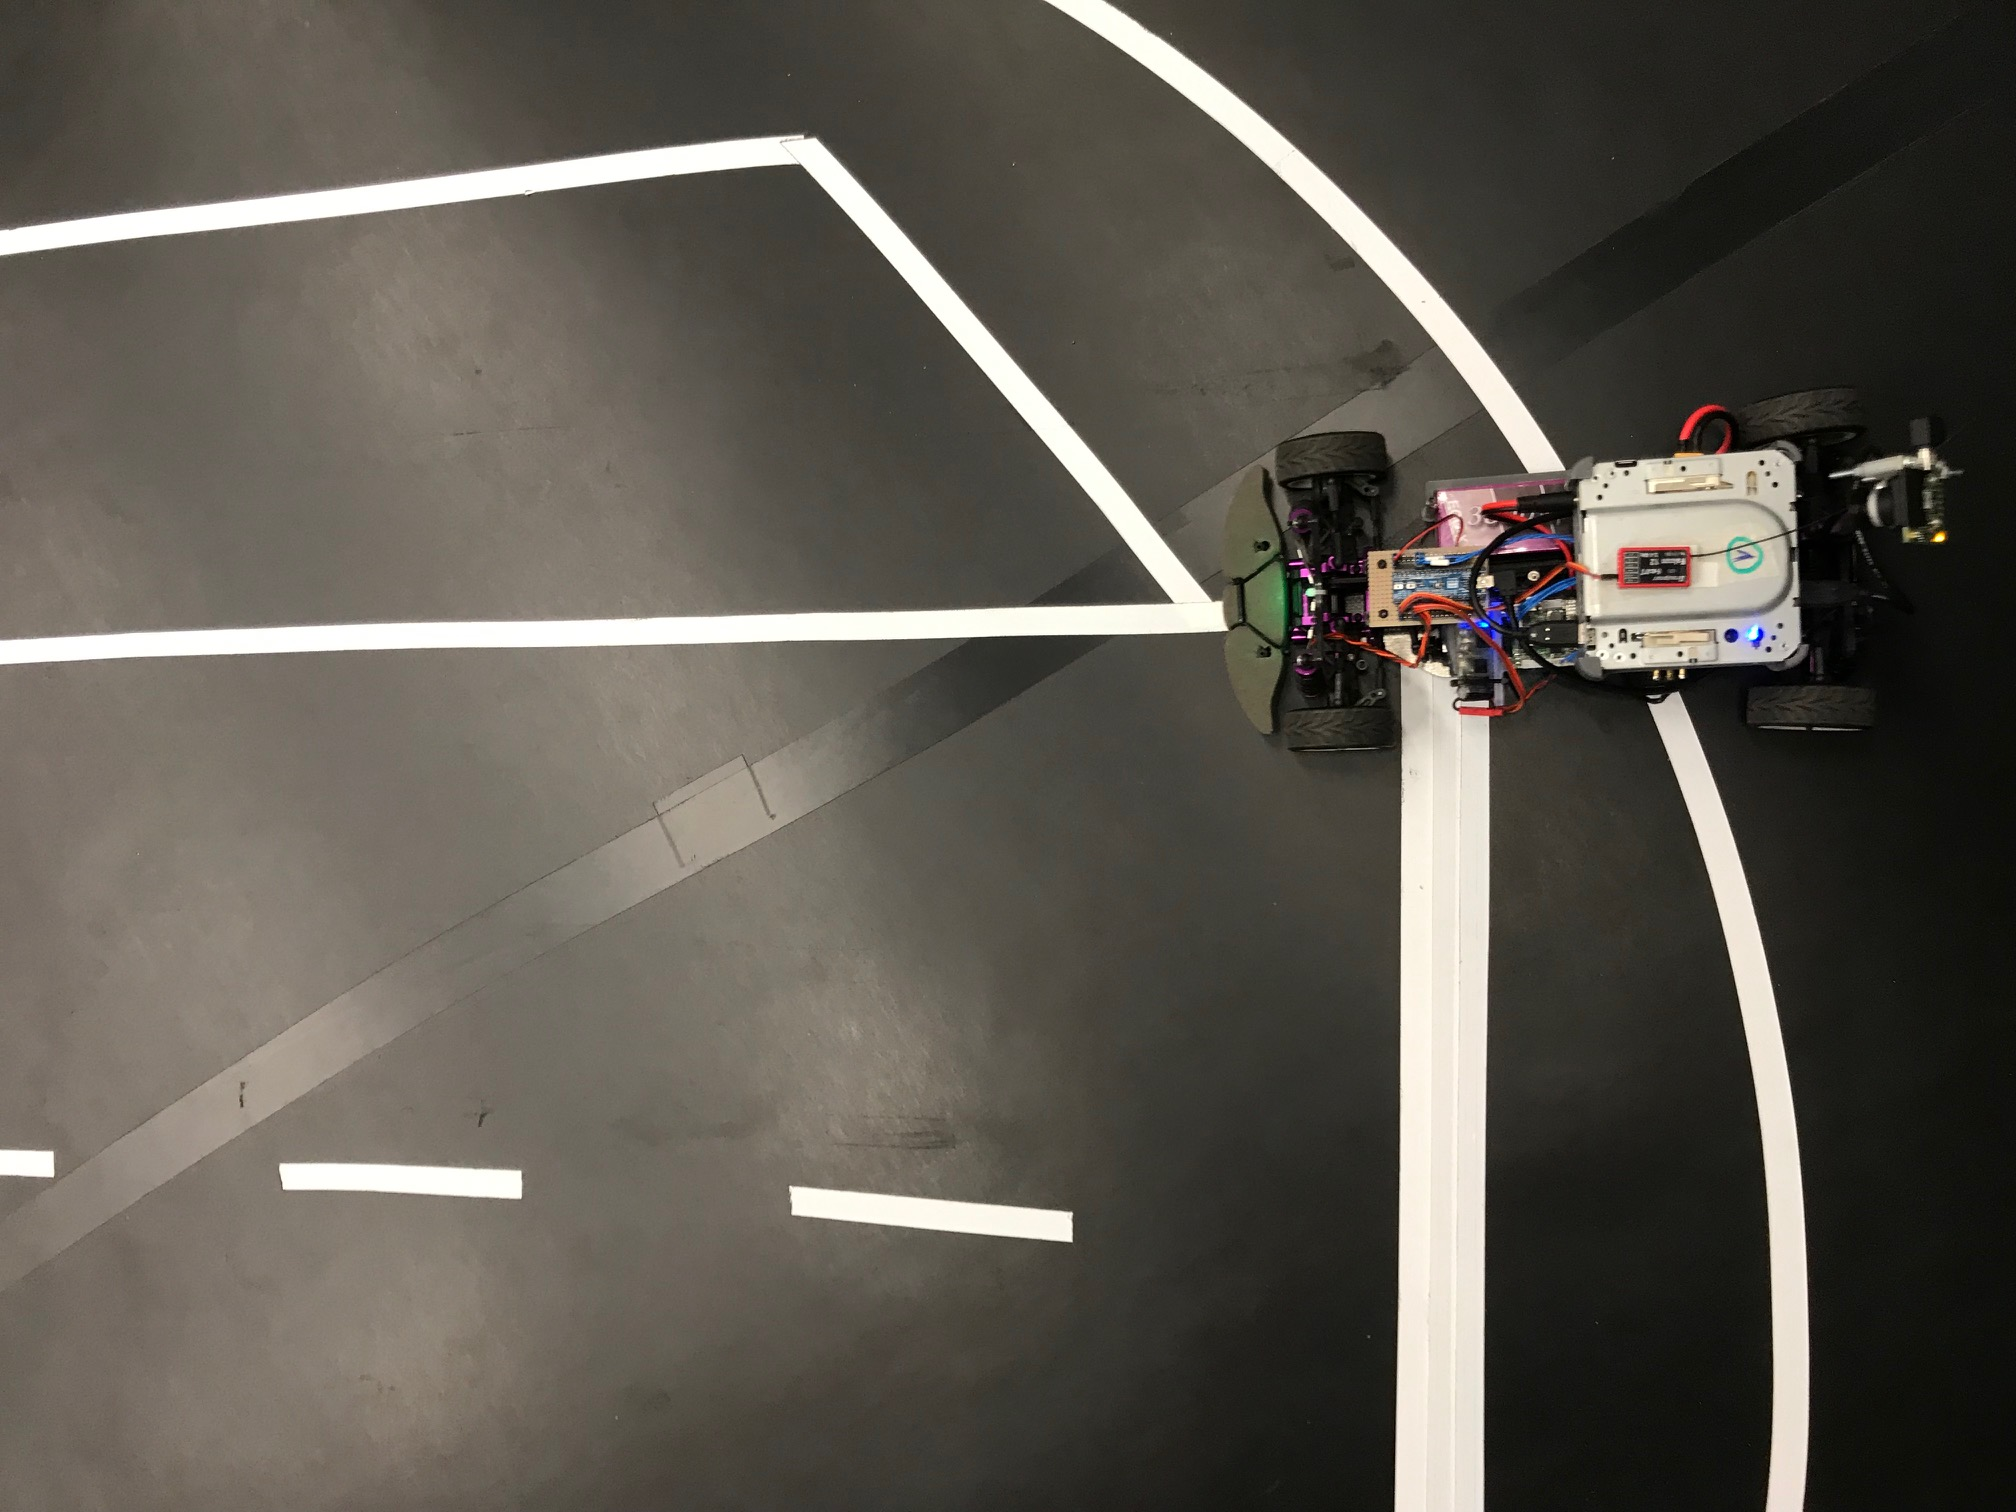
\includegraphics[width=0.8\linewidth]{figures/szenario1.jpg}
	 	  \caption{}
		  \label{fig:szena}
	\end{subfigure}%
	\begin{subfigure}{.5\textwidth}
	\centering
		  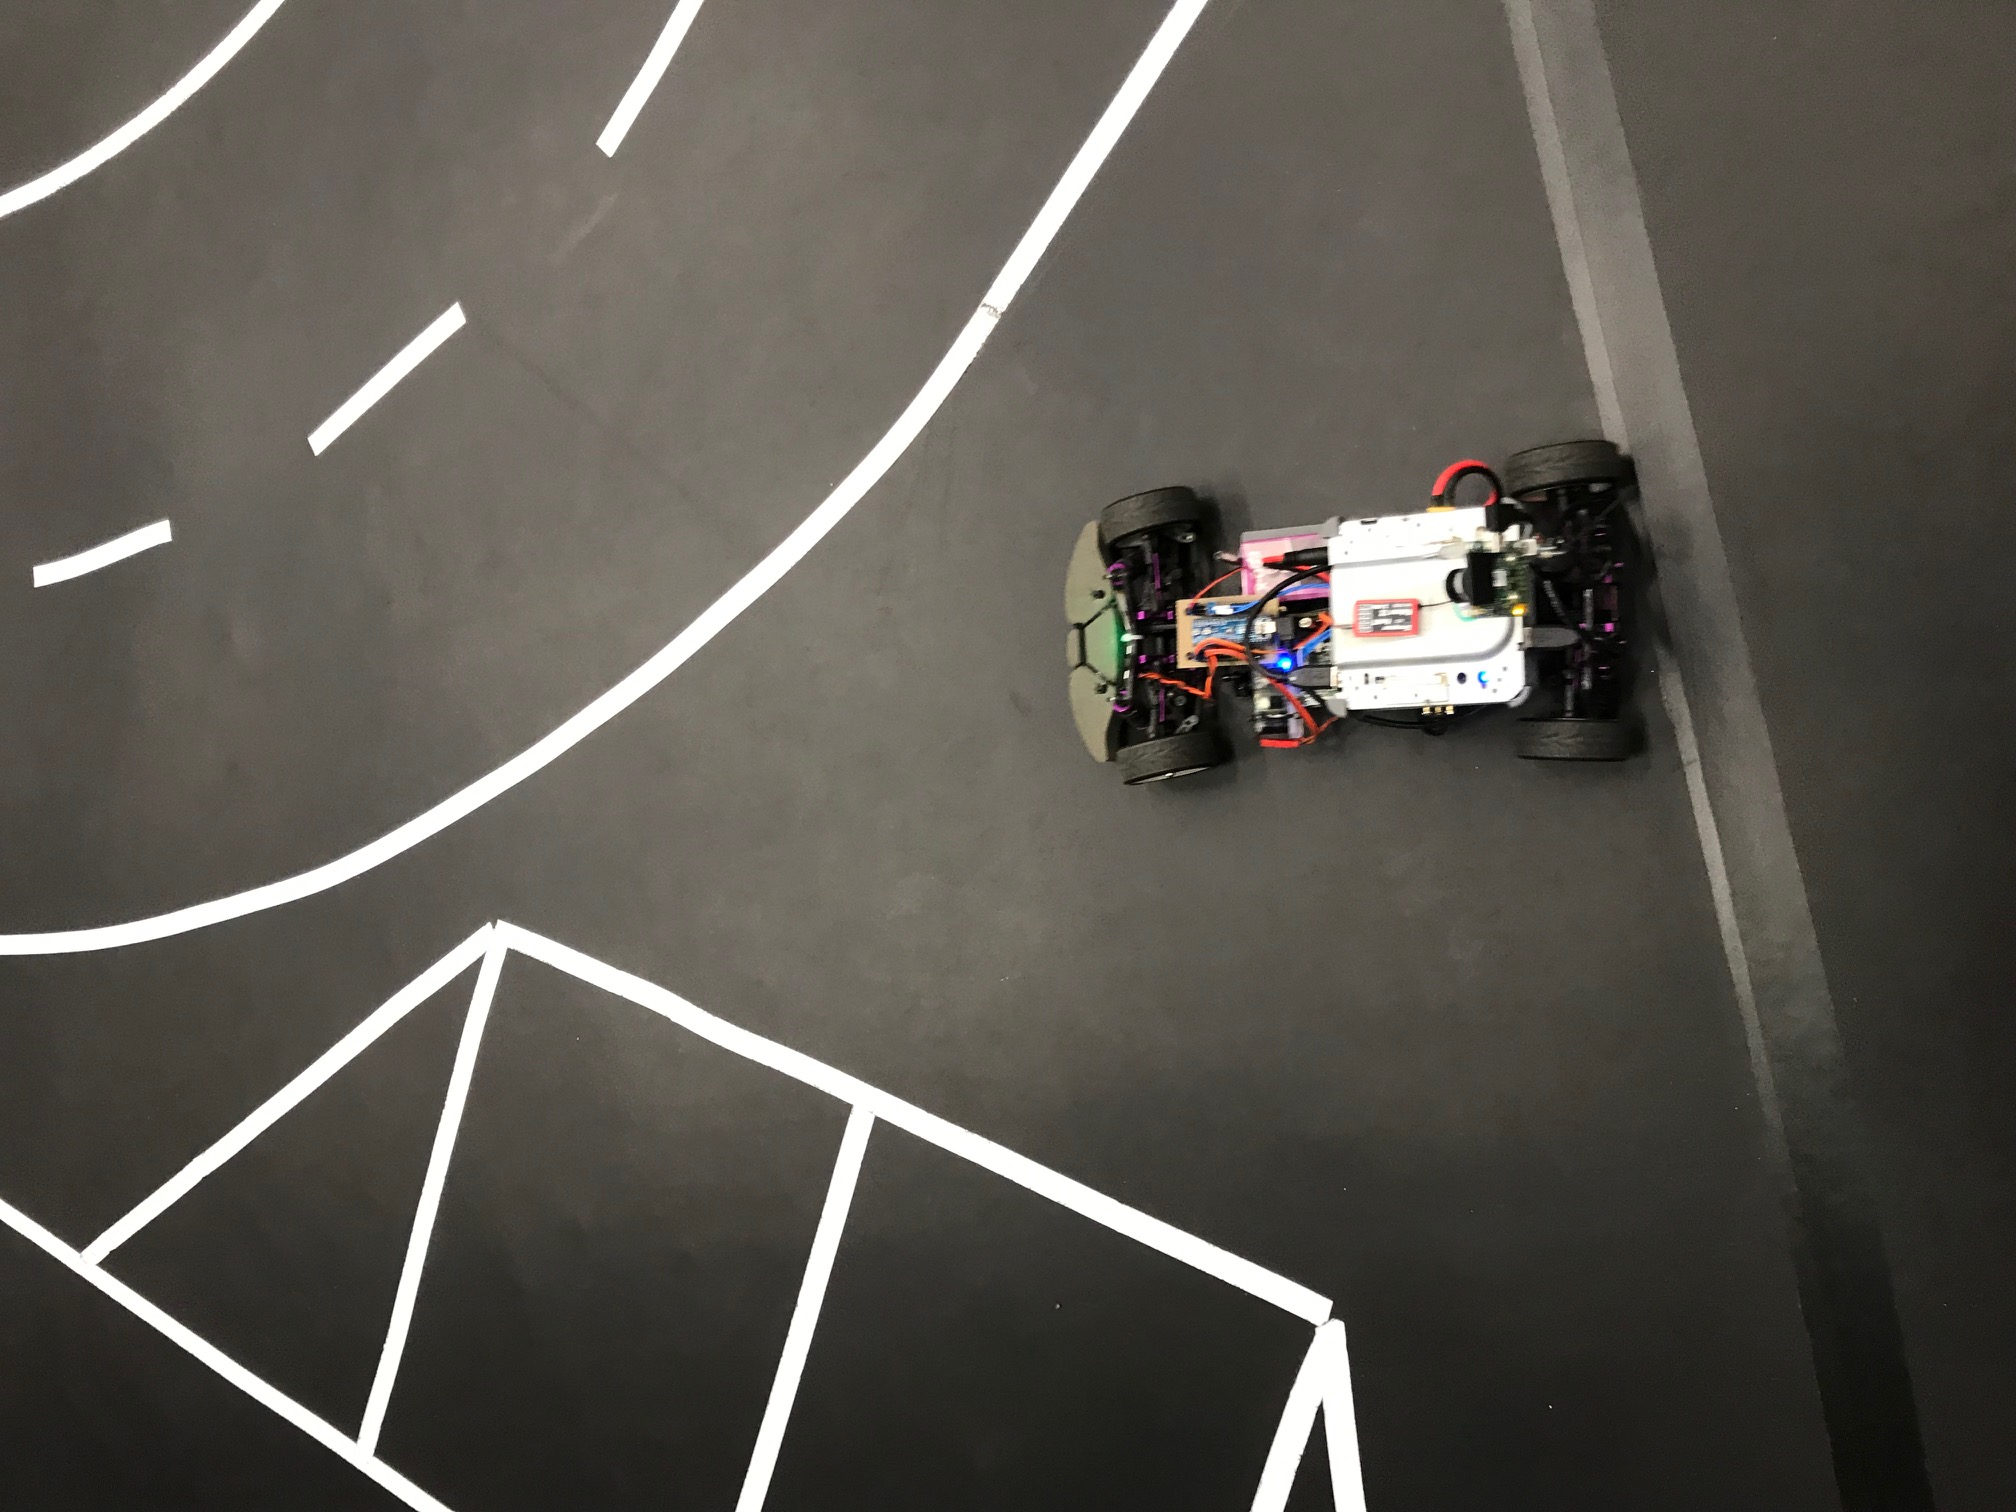
\includegraphics[width=0.8\linewidth]{figures/szenario2.jpg}
	 	  \caption{}
		  \label{fig:szenb}
	\end{subfigure}%
	\caption{Fehlerszenarien}
	\label{fig:fehlerszenarien}
\end{figure}%

Es wurden jeweils $10$ verschiedene Szenarien mit dem Fahrzeug teilweise auf der Fahrbahn und $10$ mit dem Fahrzeug außerhalb der Fahrbahn (jedoch mit Kamerasicht auf zumindest einen Teil der Fahrbahn) getestet. In $10/10$ Szenarien findet das Fahrzeug den Weg auf die Fahrspur, wenn es teilweise darauf steht. In $9/10$ Fällen findet es die Fahrspur, wenn es vollständig außerhalb der Fahrbahn steht.

Aus diesem Versuch lässt sich die Vermutung ableiten, dass die Orientierung an Fahrbahneigenschaften nicht nur in den trainierten Fällen funktioniert. Die Fahrspur wird auch aus vorher nicht gesehenen Blickwinkeln gefunden.

\paragraph{Kreuzung}
Da die Teststrecke nur eine Kreuzung hat, sind in den Traningsdaten sind nur wenige Bilder von Kreuzungsszenarien, wie dem in Abbildung~\ref{img:szenariokreuzung} gezeigten, vorhanden. Das Verhalten in diesen speziellen Situationen, in denen ein Teil der Fahrbahnmarkierung fehlt, ist besonders interessant.

\begin{figure}[h]
	\centering
	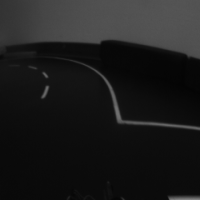
\includegraphics[scale=0.7]{figures/szenarioKreuzung.png}
	\caption{Kreuzungsszenario aus Sicht der Fahrzeugkamera}
	\label{img:szenariokreuzung}
\end{figure}

Tatsächlich erweisen sich die Kreuzungssituationen als größte Fehlerquelle. Wird die Kreuzung gerade angefahren, wird sie in $9/10$ Versuchen sauber überquert. Ist das Fahrzeug allerdings nicht mittig auf der Fahrbahn, sondern fährt die Kreuzung in einem leicht veränderten Winkel an, wird sie nur noch in $5/10$ Versuchen sauber durchfahren. In $50 \%$ der Testfälle mit leicht verändertem Blickwinkel verlässt das Fahrzeug die Fahrspur und wechselt die Spur.

Fehlt die Seitenlinie zur Orientierung, erschwert das die Lenkwinkelbestimmung. Durch eine leicht schräge Anfahrt der Kreuzung (zum Beispiel nach einer nicht ganz sauber durchfahrenen Kurve) gerät schnell die andere Fahrbahn in den Blickwinkel, welche dann zur Orientierung verwendet wird. Das Fahrzeug wechselt die Fahrspur.


\section{Visualisierung}
\paragraph{Saliency}
Gerade vor dem Hintergrund der Analyse des Netzes  ist es interessant zu Wissen, welche Bereiche des Bildes für die Bestimmung des Lenkwinkels tatsächlich von Bedeutung sind. Als Mensch kennt man das Konzept einer Fahrbahnmarkierung und der daraus entstehenden Fahrspur sehr genau. Man könnte davon ausgehen, dass für ein neuronales Netz diese Bereiche eines Bildes deswegen ebenfalls besonders interessant sind, um die Fahrtrichtung zu bestimmen.

Auch in Bezug auf die in vorangegangenem Kapitel besprochenen Problematiken liegt ein gesteigertes Interesse vor, die wichtigen Bereiche der Fahrbahnbilder ausfindig zu machen.

Für die Visualisierung werden so genannte Saliency-Maps verwendet. Diese wurden 2013 in einem Papert \cite{simonyan2013deep} erstmals vorgestellt. Die Idee ist, jene Bildpunkte zu identifizieren, welche für die größten Veränderungen im Output sorgen. Für diese Arbeit bedeutet das, genau die Bildpunkte visuell hervorzuheben, welche für eine große Veränderung im Lenkwinkeloutput sorgen. Dafür wird die Veränderung (Gradient) des Outputs (Lenkwinkel) in Bezug auf das Eingabebild berechnet, also das Verhältnis einer Änderung im Output zu einer Änderung im Input: $\frac{\partial Output}{\partial Input}$.    Für diese Analyse wird Keras-vis \citeI{raghakotkerasvis} genutzt, eine Visualisierungs-API für Keras.

Um die Repräsentation der Bildeigenschaften im Netz deutlich zu machen, wird eine Saliency Map für jeden der drei Residual-Blöcke bestimmt. So lässt sich nachvollziehen, wie sich die ausschlaggebenden Bildbereiche auf dem Weg durch das Netz verändern. In Abbildung~\ref{img:saliency} sind diese drei Saliency Maps für ein Beispielbild einer Linkskurve dargestellt.

Die hellen Bildbereiche sind eben die, die für eine Erhöhung des Outputs sorgen, also für einen positiven Lenkwinkel. Zur Erinnerung, ein positiver Lenkwinkel codiert eine Linkskurve. Die Saliency-Map wurde für die jeweils letzte Convolutional-Layer des Blocks berechnet.

\begin{figure}
	\centering
	\begin{subfigure}{\textwidth}
	\centering
		  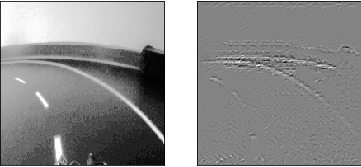
\includegraphics[width=0.8\linewidth]{figures/firstBlock.png}
	 	  \caption{Residual-Block 1}
		  \label{fig:saliena}
	\end{subfigure}\\
	\begin{subfigure}{\textwidth}
	\centering
		  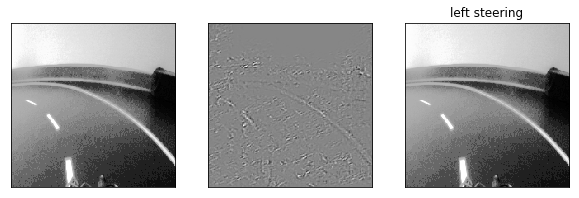
\includegraphics[width=0.8\linewidth]{figures/secondBlock.png}
	 	  \caption{Residual Block 2}
		  \label{fig:salienb}
	\end{subfigure}\\
	\begin{subfigure}{\textwidth}
	\centering
		  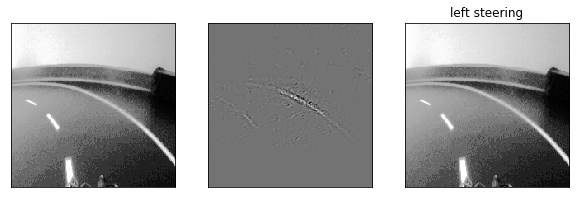
\includegraphics[width=0.8\linewidth]{figures/thirdBlock.png}
	 	  \caption{Residual Block 3}
		  \label{fig:salienc}
	\end{subfigure}%
	\caption{Ausschlaggebende Bildbereiche}
	\label{img:saliency}
\end{figure}%

Zu sehen ist jeweils das Bild der Fahrbahn nach einem Histogrammausgleich, rechts daneben die berechnete Saliency-Map. Nach dem ersten Residual Block \ref{fig:saliena} scheint die Aufmerksamkeit insbesondere auf linienartigen Bereichen zu liegen, gut zu sehen an der hellen Hervorhebung der Bildpunkte. Neben der Fahrbahnbegrenzung spielt auch ein Teil der Wandlinien eine Rolle für die Bestimmung der Linkslenkung. In \ref{fig:salienb}, nach der letzten Convolutional-Layer des zweiten Residual-Blocks, zeigt sich eine Veränderung. Die Ausprägung der Linienstrukturen in der Saliency-Map beschränkt sich auf die Fahrbahnmarkierung, die unterbrochene Mittellinie tritt etwas deutlicher hervor. Insgesamt wirkt die Verteilung der prägnanten Bildbereiche zufälliger, fast wie ein Rauschen.
Nach dem dritten und letzten Residual-Block \ref{fig:salienc} liegt der Aufmerksamkeitsfokus auf einem Stück der Außenlinie.  Die Bildpunkte, die hier liegen, sind die Entscheidenden für die Linkslenkung (Lenkwinkel $\interval{0}{1}$). Hier muss Berücksichtigt werden, dass nur der letzte Residual-Block von Anpassungen der Filter betroffen war. Die starke Konzentration auf den Abschnitt der Außenlinie ist darauf zurückzuführen.

\paragraph{Kreuzung}
Die angesprochene Schwierigkeit von Kreuzungssituationen wird mithilfe von Saliency-Maps noch einmal neu betrachtet. In Abbildung~\ref{img:kreuzung} ist das Kreuzungsbild der Saliency-Map gegenüber gestellt.

\begin{figure}[h]
	\centering
	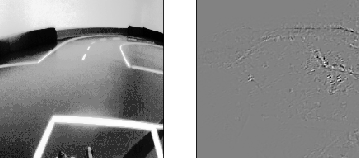
\includegraphics[scale=1.3]{figures/Kreuzung.png}
	\caption{Saliency-Map einer Kreuzungssituation}
	\label{img:kreuzung}
\end{figure}

Es ist zu erkennen, dass besonders die Ecke der sich treffenden Fahrbahnlinien der gegenüberliegenden Seite hervortritt. Außerdem zeichnet sich die Außenlinie der linken Fahrbahnseite hinter der Kreuzung ab.

Positiv ist, dass trotz fehlender Fahrbahnbegrenzung die entfernten Linien hinter der Kreuzung als Orientierung genutzt werden. Allerdings lässt sich in diesem Beispiel auch die Spurwechsel-Problematik erkennen. \note{Erklärung unvollständig}



\input{chapters/6-Resümee}



%\bibliographystyle{plain}
%Paper (also books etc.)
\bibliographystyle{dinat}
\bibliography{literature}

%Internet
\bibliographystyleI{dinat}
\bibliographyI{internet}


% Appendix
%\appendix
%% !TEX root = ../thesis.tex
% appendix example chapter
% @author Thomas Lehmann
%
\chapter{Anhang}


\IGlossary


\Istatement

\end{document}
